% SPDX-FileCopyrightText: Copyright (c) 2026 Newton Developers
% SPDX-License-Identifier: CC-BY-4.0
\documentclass[10pt]{article}
\usepackage[margin=18mm]{geometry}
\usepackage{graphicx,booktabs,longtable,hyperref}
\title{Alpha box benchmark: 3--10 m terrain}
\date{September 28, 2026}
\begin{document}
\maketitle
The updated alpha box example uses two-way coupling and a dynamic box following a
0.2 m/s force-controlled reference. Background sizes are 3--10 m square.
Moving-patch uses 2 m square simulated terrain plus a 0.5 m boundary on each side.
Fixed and sparse use full-size particle beds. Sand depth is 0.5 m; voxel size is
0.05 m; sampling is 3 particles per voxel axis. Density is 2500 kg/m$^3$, Young's
modulus 40 MPa, Poisson's ratio 0.3, and friction $\tan(50^\circ)$.
PIC transfer, P0 strain, Q1 velocity, S2 collider, automatic warmstart and at most
50 iterations are used. These controlled settings match the earlier benchmark,
rather than the interactive defaults. Execution is headless at 200 Hz with four
rigid substeps, without outer CUDA graph capture, on an RTX 5090.

Two fresh-process repeats each use 150 warm-up and 150 measured steps.
Physics timings include a GPU synchronization. Error bars are mean plus/minus
sample standard deviation of pooled steps. VRAM is sampled device-wide memory
minus the pre-CUDA baseline, every 50 ms; desktop activity affects this estimate.
Peak includes initialization and warm-up. Shorter peaks can be missed.
Missing points are failed cases, not zero cost. Source hashes and full settings
are included with the data. This short-run benchmark does not establish
long-distance locomotion stability.
\begin{figure}[h]\centering
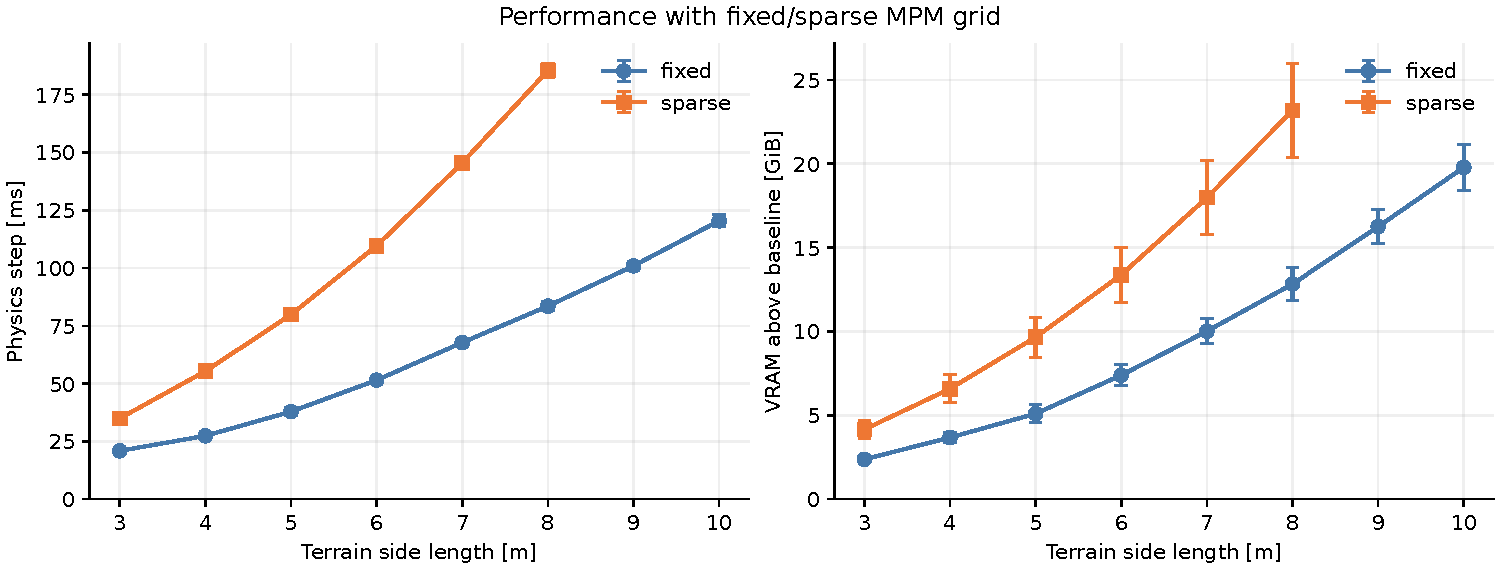
\includegraphics[width=\linewidth]{01_grid_comparison.pdf}
\end{figure}
\begin{figure}[h]\centering
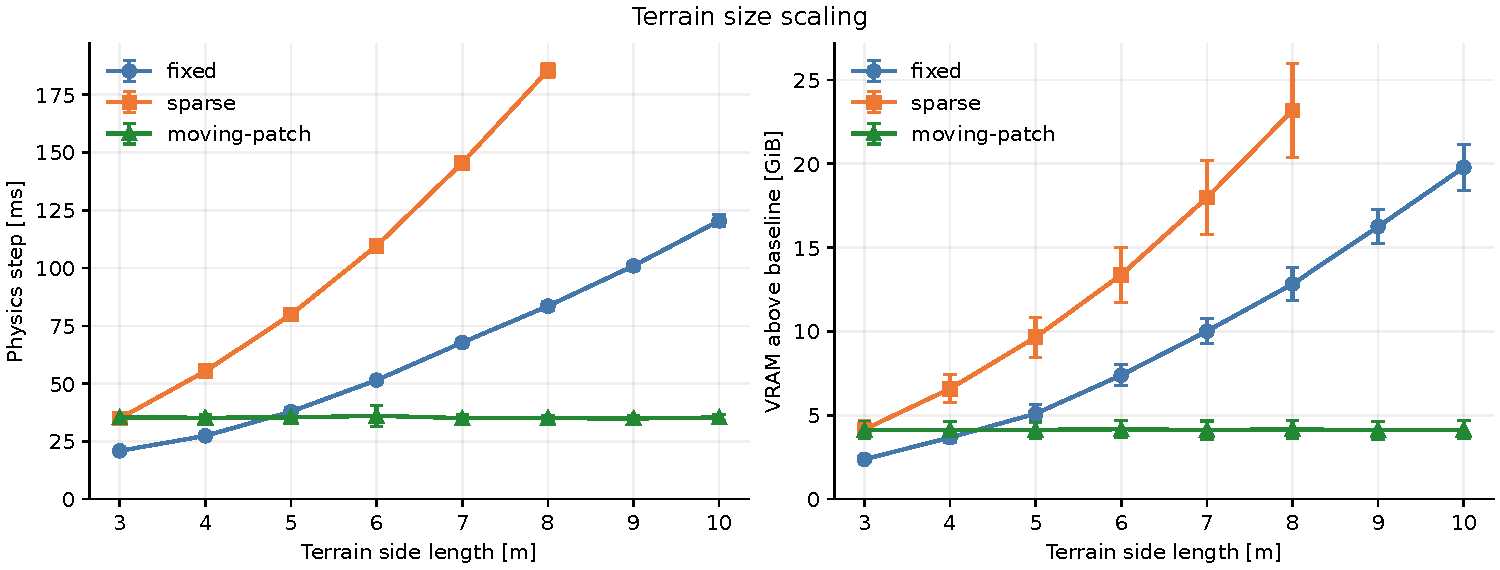
\includegraphics[width=\linewidth]{02_terrain_scaling.pdf}
\end{figure}
\clearpage
For fixed, increasing the terrain side from 3 to 10 m changes mean physics time from 20.91 to 120.46 ms and steady VRAM from 2.38 to 19.78 GiB.

For sparse, increasing the terrain side from 3 to 8 m changes mean physics time from 34.94 to 185.47 ms and steady VRAM from 4.16 to 23.18 GiB.

For moving-patch, increasing the terrain side from 3 to 10 m changes mean physics time from 35.39 to 35.37 ms and steady VRAM from 4.12 to 4.13 GiB.

Only moving-patch keeps its particle region and reserved cell capacity constant as the background grows. Fixed and sparse both simulate the full particle bed; sparse allocation does not restrict the material solve to particles touching the box. The 3 m cases have equal particle allocation, so comparing moving-patch with sparse at 3 m estimates total patch-maintenance overhead under this short-run protocol. Comparing moving-patch with fixed also includes a grid-method difference. These results concern a flat, densely filled bed and this reservation policy; they are not a claim about all sparse-grid configurations.

The box moves during the size sweep, but does not travel far enough to shift the patch center (centers are spaced 0.4 m apart) before the short run ends. No patch shifts occur during the measured interval. Per-step patch checks are timed; particle recycling during a shift is covered by the longer run below.

\paragraph{Longer moving-patch validation.}
On a 6 m background, two repeats use 150 warm-up and 1200 measured steps. Repeat 0: 35.35 $\pm$ 1.70 ms per step; 4.14 GiB steady VRAM; 2 patch shifts during the 6 s measured interval; final box X = 0.78 m.

Repeat 1: 35.39 $\pm$ 1.54 ms per step; 4.14 GiB steady VRAM; 2 patch shifts during the 6 s measured interval; final box X = 0.78 m.

\begin{longtable}{rlrrrr}
\toprule
Side [m] & Method & Repeats & Step [ms] & Steady [GiB] & Peak [GiB] \\
\midrule\endhead
3 & fixed & 2/2 & 20.91 $\pm$ 1.07 & 2.38 $\pm$ 0.15 & 2.64 \\
3 & moving-patch & 2/2 & 35.39 $\pm$ 1.70 & 4.12 $\pm$ 0.53 & 4.91 \\
3 & sparse & 2/2 & 34.94 $\pm$ 1.28 & 4.16 $\pm$ 0.52 & 4.95 \\
4 & fixed & 2/2 & 27.40 $\pm$ 1.36 & 3.67 $\pm$ 0.27 & 4.00 \\
4 & moving-patch & 2/2 & 35.24 $\pm$ 1.39 & 4.12 $\pm$ 0.51 & 4.91 \\
4 & sparse & 2/2 & 55.37 $\pm$ 1.79 & 6.58 $\pm$ 0.83 & 7.63 \\
5 & fixed & 2/2 & 37.88 $\pm$ 1.62 & 5.10 $\pm$ 0.54 & 5.82 \\
5 & moving-patch & 2/2 & 35.37 $\pm$ 1.27 & 4.14 $\pm$ 0.52 & 4.97 \\
5 & sparse & 2/2 & 79.85 $\pm$ 2.09 & 9.66 $\pm$ 1.19 & 11.03 \\
6 & fixed & 2/2 & 51.51 $\pm$ 1.50 & 7.39 $\pm$ 0.63 & 7.99 \\
6 & moving-patch & 2/2 & 36.07 $\pm$ 4.44 & 4.17 $\pm$ 0.51 & 5.00 \\
6 & sparse & 2/2 & 109.67 $\pm$ 2.71 & 13.38 $\pm$ 1.63 & 15.15 \\
7 & fixed & 2/2 & 67.77 $\pm$ 1.57 & 10.01 $\pm$ 0.75 & 10.59 \\
7 & moving-patch & 2/2 & 35.08 $\pm$ 1.44 & 4.13 $\pm$ 0.54 & 4.94 \\
7 & sparse & 2/2 & 145.55 $\pm$ 2.79 & 17.98 $\pm$ 2.21 & 20.07 \\
8 & fixed & 2/2 & 83.54 $\pm$ 1.93 & 12.83 $\pm$ 0.97 & 13.56 \\
8 & moving-patch & 2/2 & 35.05 $\pm$ 1.22 & 4.16 $\pm$ 0.53 & 4.91 \\
8 & sparse & 2/2 & 185.47 $\pm$ 3.17 & 23.18 $\pm$ 2.79 & 25.66 \\
9 & fixed & 2/2 & 100.97 $\pm$ 1.84 & 16.25 $\pm$ 1.02 & 16.90 \\
9 & moving-patch & 2/2 & 34.90 $\pm$ 1.18 & 4.11 $\pm$ 0.53 & 4.91 \\
9 & sparse & 0/2 & failed & failed & failed \\
10 & fixed & 2/2 & 120.46 $\pm$ 2.60 & 19.78 $\pm$ 1.38 & 20.66 \\
10 & moving-patch & 2/2 & 35.37 $\pm$ 1.32 & 4.13 $\pm$ 0.53 & 4.92 \\
10 & sparse & 0/2 & failed & failed & failed \\
\bottomrule\end{longtable}
Complete failure details and per-case particle and cell counts are in README.md and summary.csv.
\end{document}
